% Options for packages loaded elsewhere
\PassOptionsToPackage{unicode}{hyperref}
\PassOptionsToPackage{hyphens}{url}
%
\documentclass[
]{article}
\usepackage{amsmath,amssymb}
\usepackage{lmodern}
\usepackage{iftex}
\ifPDFTeX
  \usepackage[T1]{fontenc}
  \usepackage[utf8]{inputenc}
  \usepackage{textcomp} % provide euro and other symbols
\else % if luatex or xetex
  \usepackage{unicode-math}
  \defaultfontfeatures{Scale=MatchLowercase}
  \defaultfontfeatures[\rmfamily]{Ligatures=TeX,Scale=1}
\fi
% Use upquote if available, for straight quotes in verbatim environments
\IfFileExists{upquote.sty}{\usepackage{upquote}}{}
\IfFileExists{microtype.sty}{% use microtype if available
  \usepackage[]{microtype}
  \UseMicrotypeSet[protrusion]{basicmath} % disable protrusion for tt fonts
}{}
\makeatletter
\@ifundefined{KOMAClassName}{% if non-KOMA class
  \IfFileExists{parskip.sty}{%
    \usepackage{parskip}
  }{% else
    \setlength{\parindent}{0pt}
    \setlength{\parskip}{6pt plus 2pt minus 1pt}}
}{% if KOMA class
  \KOMAoptions{parskip=half}}
\makeatother
\usepackage{xcolor}
\usepackage{longtable,booktabs,array}
\usepackage{calc} % for calculating minipage widths
% Correct order of tables after \paragraph or \subparagraph
\usepackage{etoolbox}
\makeatletter
\patchcmd\longtable{\par}{\if@noskipsec\mbox{}\fi\par}{}{}
\makeatother
% Allow footnotes in longtable head/foot
\IfFileExists{footnotehyper.sty}{\usepackage{footnotehyper}}{\usepackage{footnote}}
\makesavenoteenv{longtable}
\usepackage{graphicx}
\makeatletter
\def\maxwidth{\ifdim\Gin@nat@width>\linewidth\linewidth\else\Gin@nat@width\fi}
\def\maxheight{\ifdim\Gin@nat@height>\textheight\textheight\else\Gin@nat@height\fi}
\makeatother
% Scale images if necessary, so that they will not overflow the page
% margins by default, and it is still possible to overwrite the defaults
% using explicit options in \includegraphics[width, height, ...]{}
\setkeys{Gin}{width=\maxwidth,height=\maxheight,keepaspectratio}
% Set default figure placement to htbp
\makeatletter
\def\fps@figure{htbp}
\makeatother
\setlength{\emergencystretch}{3em} % prevent overfull lines
\providecommand{\tightlist}{%
  \setlength{\itemsep}{0pt}\setlength{\parskip}{0pt}}
\setcounter{secnumdepth}{5}
\newlength{\cslhangindent}
\setlength{\cslhangindent}{1.5em}
\newlength{\csllabelwidth}
\setlength{\csllabelwidth}{3em}
\newlength{\cslentryspacingunit} % times entry-spacing
\setlength{\cslentryspacingunit}{\parskip}
\newenvironment{CSLReferences}[2] % #1 hanging-ident, #2 entry spacing
 {% don't indent paragraphs
  \setlength{\parindent}{0pt}
  % turn on hanging indent if param 1 is 1
  \ifodd #1
  \let\oldpar\par
  \def\par{\hangindent=\cslhangindent\oldpar}
  \fi
  % set entry spacing
  \setlength{\parskip}{#2\cslentryspacingunit}
 }%
 {}
\usepackage{calc}
\newcommand{\CSLBlock}[1]{#1\hfill\break}
\newcommand{\CSLLeftMargin}[1]{\parbox[t]{\csllabelwidth}{#1}}
\newcommand{\CSLRightInline}[1]{\parbox[t]{\linewidth - \csllabelwidth}{#1}\break}
\newcommand{\CSLIndent}[1]{\hspace{\cslhangindent}#1}
\usepackage{booktabs}

\usepackage{longtable}
\usepackage{array}
\usepackage{multirow}
\usepackage{wrapfig}
\usepackage{float}
\usepackage{colortbl}
\usepackage{pdflscape}
\usepackage{tabu}
\usepackage{threeparttable}
\usepackage{threeparttablex}
\usepackage[normalem]{ulem}
\usepackage[utf8]{inputenc}
\usepackage{makecell}
\usepackage{xcolor}
\usepackage{siunitx}
\usepackage{booktabs}
\usepackage{longtable}
\usepackage{array}
\usepackage{multirow}
\usepackage{wrapfig}
\usepackage{float}
\usepackage{colortbl}
\usepackage{pdflscape}
\usepackage{tabu}
\usepackage{threeparttable}
\usepackage{threeparttablex}
\usepackage[normalem]{ulem}
\usepackage{makecell}
\usepackage{xcolor}
\ifLuaTeX
  \usepackage{selnolig}  % disable illegal ligatures
\fi
\IfFileExists{bookmark.sty}{\usepackage{bookmark}}{\usepackage{hyperref}}
\IfFileExists{xurl.sty}{\usepackage{xurl}}{} % add URL line breaks if available
\urlstyle{same} % disable monospaced font for URLs
\hypersetup{
  pdftitle={Modeling and Analysis of On-Demand Transit in Salt Lake County Using BEAM},
  pdfkeywords={Accessibility,, Microtransit,, Passive Data,, Location Choice},
  hidelinks,
  pdfcreator={LaTeX via pandoc}}

\title{Modeling and Analysis of On-Demand Transit in Salt Lake County Using BEAM}
\author{true \and true}
\date{2022-10-18}

\begin{document}
\maketitle
\begin{abstract}
A number of regions have begun operating microtransit systems to support first and last mile transit access. In this paper, we modify the ridehailing request handling algorithm in the BEAM microscopic simulation engine to accomodate geographically resetricted microstransit operations. We then examine the ridership operating characteristics for one existing and three proposed geofenced service regions in Salt Lake County, Utah. We find that the simulation generates realistic ridership statistics and wait times, subject to errors likely to be corrected with more thorough choice model calibration. We also found that expanding microtransit services to Sandy or West Jordan might be effective, but might be less so for the area near SLC International Airport.
\end{abstract}

{
\setcounter{tocdepth}{2}
\tableofcontents
}
\hypertarget{introduction}{%
\section{Introduction}\label{introduction}}

\hypertarget{problem-statement}{%
\subsection{Problem Statement}\label{problem-statement}}

In November of 2019, the Utah Transit Authority (UTA) began a partnership with VIA, a private mobility company. Under this partnership, UTA has supplemented its fixed-route services in south Salt Lake County with on-demand shuttles hailed through a mobile application. So-called ``microtransit'' offerings of this kind have the potential to efficiently extend UTA services into low-density areas and function as last-mile services for the regular fixed-route rail and bus network. UTA is interested in examining other areas where microtransit services can be effectively deployed.

In September 2020, UTA released a report detailing a possible expansion of microtransit services to other areas in Utah following the UTA on Demand pilot program (\protect\hyperlink{ref-UTAreport}{Robertson et al., 2020}). 19 zones were identified between Brigham City and Santaquin as areas that could potentially benefit from microtransit services. Ridership was estimated based on number of residents and number of workers employed within each zone, as well as a mode share score that VIA developed based on their internal demand model.

We seek however to provide UTA and the Utah Department of Transportation (UDOT) with a microsimulation model they can use as a template to examine future similar projects. We want to know how the results of such a model would compare to those of UTA's September 2020 report. Though UTA's own report made no definitive recommendations regarding expansion of microtransit services, it may be useful in calibrating our simulation. We also seek to use our results (possibly in conjunction with those of UTA's report) to make recommendations to UTA and UDOT regarding expansion of microtransit services.

\hypertarget{objectives}{%
\subsection{Objectives}\label{objectives}}

The primary objective of this research project is to identify possible geographic areas along the Wasatch Front where an on-demand microtransit system might most effectively operate. To do this, the research team will implement an on-demand microtransit system within a multi-agent simulation of daily activity patterns for the Wasatch Front Region. This simulation is presently under construction for other UDOT-sponsored research projects aimed at evaluating the potential effects of an on-demand transit system aimed at wheelchair users, and an additional USDOT-funded project to examine techniques to optimize microtransit services.

A secondary objective of this research will be to provide a template for UDOT and UTA to examine projects of this kind with a microsimulation model. Utah has invested a great deal of resources into fixed route, high-capacity transit lines such as UVX, TRAX, and FrontRunner. These services perform well and have relatively high ridership statistics, but many people not directly near the stations can have difficulty accessing them. UTA will use this research to identify other places on the Wasatch Front where microtransit offerings could be successful. UDOT could also use this methodology to study the potential effectiveness of such services in other areas, such as Logan, Moab, and Cedar City.

\hypertarget{scope}{%
\subsection{Scope}\label{scope}}

This analysis is being developed using BEAM: the modeling framework for Behavior, Energy, Autonomy, and Mobility developed by Lawrence Berkeley National Laboratory. This research takes the BEAM model as given, modifying only those parameters and implementations that are necessary to conduct the current analysis. For example, we will modify the BEAM code to enable geo-fenced microtransit operations, which are a critical component of the current research. We will not attempt to modify BEAM's multi-modal pathfinding algorithms, which may affect the current research but must be taken as given under the scope of this project.

\hypertarget{outline-of-report}{%
\subsection{Outline of Report}\label{outline-of-report}}

The report is organized into the following chapters:

\begin{enumerate}
\def\labelenumi{\arabic{enumi}.}
\tightlist
\item
  \textbf{Introduction:} This chapter.
\item
  \textbf{Literature Review:} An overview of previous efforts to understand microtransit systems and forecast their operations.
\item
  \textbf{Methodology:} Methods and data used to create the initial microsimulation scenario in the Salt Lake City region.
\item
  \textbf{Results:} A comparison of initial BEAM modeling to observed data, and an evaluation of three additional regions selected by UTA and UDOT for simulation analysis.
\item
  \textbf{Recommendations and Conclusions}
\end{enumerate}

\hypertarget{literature-review}{%
\section{Literature Review}\label{literature-review}}

\hypertarget{overview}{%
\subsection{Overview}\label{overview}}

This chapter presents prior attempts in the academic and practical literature to understand, model, and predict ridership for on-demand transit systems. The literature highlights the power and flexibility of demand-based modeling. MATSim is an agent-based simulation that models individuals' behavior, and BEAM (an extension to MATSim) places even more focus on individuals. As our project deals with modeling the UTA on Demand by VIA pilot program in Salt Lake City, we additionally discuss the program and the results it has achieved so far. Ultimately, we conclude that we will be using BEAM to model this and other potential on-demand transit implementations.

\hypertarget{purposes-and-description-of-on-demand-transit}{%
\subsection{Purposes and Description of On-Demand Transit}\label{purposes-and-description-of-on-demand-transit}}

One aspect of traditional public transit is that the routes are usually fixed. It is not always feasible to extend these fixed-route systems into less densely populated areas (at least, not in a way that would reasonably service most of the residents) due to the high costs of capital and operation and the relatively low ridership that would result (\protect\hyperlink{ref-MinetaTransportationInstitute2012}{Institute, 2012}). However, public transit has many benefits such as reduced carbon emissions per person-mile and less traffic congestion (\protect\hyperlink{ref-Buchanan2019}{Buchanan, 2019}; \protect\hyperlink{ref-Gershon2005}{Gershon, 2005}), and the lack of transit options in many suburban areas requires residents to overwhelmingly use personal vehicles as their main form of transportation (\protect\hyperlink{ref-Gershon2005}{Gershon, 2005}). This raises the question of the most effective and efficient way to increase transit ridership and decrease dependence on personal vehicles in these areas.

One possible solution is the introduction of microtransit services. Microtransit is a form of shared, on-demand transportation (ODT) in which passengers schedule rides and vehicle routing is updated in real time to efficiently transport its users. The vehicles used are usually a form of minibus that can hold several passengers at once (\protect\hyperlink{ref-Shaheen2015}{Shaheen et al., 2015}). One key application of microtransit is for first- and last-mile transportation, connecting a wide area to the existing fixed-route network (\protect\hyperlink{ref-Shaheen2015}{Shaheen et al., 2015}) and taking less time than walking or cycling. Decreasing this first/last mile travel time can increase job accessibility by allowing individuals to travel farther with the same travel time budget, and some microtransit services have been shown to decrease this time significantly (\protect\hyperlink{ref-Kang2019}{Kang and Hamidi, 2019}). Especially as smartphone ownership and usage continues to increase, microtransit is a promising option, as booking rides can be done within phone apps, making the user experience easier (\protect\hyperlink{ref-Agatz2011}{Agatz et al., 2011}).

\hypertarget{analysis-framework}{%
\subsubsection{Analysis framework}\label{analysis-framework}}

Alonso-González et al. (\protect\hyperlink{ref-Alonso-Gonzalez2018}{2018}) set out to create an analysis framework that can be used to evaluate ODT services, both in simulation and real-world application, in order to compare them to existing systems. The framework presented requires identifying several characteristics of the ODT system: coverage and routing, operating hours, vehicle characteristics, the booking system, and request acceptance criteria. Then several quantities are calculated or estimated, including generalized journey time and share of declined ODT trips as well as usage values. The ODT system is then compared with other modes such as fixed transit and walking/biking. The study concludes that a generalized cost of travel metric would be the most useful in comparing the ODT system against other options, as it was a good indicator of changes in mobility.

\hypertarget{previous-attempts-to-model-on-demand-transit}{%
\subsection{Previous Attempts to Model On-Demand Transit}\label{previous-attempts-to-model-on-demand-transit}}

Due to the high potential of ODT/microtransit services, many models and simulations have been created. Vosooghi et al. (\protect\hyperlink{ref-Vosooghi2017}{2017}) published a literature review discussing several simulation software packages: Azevedo et al. (\protect\hyperlink{ref-Azevedo2016}{2016}) used SimMobility to model an autonomous taxi network, MobiTroop was used by Heilig et al. (\protect\hyperlink{ref-Heilig2015}{2015}) to simulate carsharing in the Stuttgart, Germany area, and MATSim has been used to develop a carsharing model in Berlin (\protect\hyperlink{ref-Ciari2014}{Ciari et al., 2014}) and analyze one in Zurich (\protect\hyperlink{ref-Balac2015}{Balać et al., 2015}), and it was used to model a shared autonomous vehicle system (\protect\hyperlink{ref-Fagnant2014}{Fagnant and Kockelman, 2014}).

Ronald et al. (\protect\hyperlink{ref-Ronald2015}{2015}) looked at three software simulations in more detail: the basic simulation Delphi, the agent-based simulation MATSim, and the traffic microsimulation SUMOoD (SUMO on Demand). The study found that these simulations generally produced similar results with respect to number of vehicles and amount of demand, and noted that all simulations performed as expected based on real-world observations (\protect\hyperlink{ref-Schofer2003}{Schofer et al., 2003}). They are also quick to point out that results of these simulations might be optimistic if simplifications to routing are made or if using an undirected network, where a vehicle could pick up passengers on either side of a road no matter the direction of travel.

\hypertarget{matsim-and-beam}{%
\subsubsection{MATSim and BEAM}\label{matsim-and-beam}}

MATSim (Multi-Agent Transport Simulation) is an open-source framework for transportation modeling originally developed in Zurich. The framework simulates traffic flows and congestion on a microscopic level, and simulates demand by creating agents and following their daily schedules and decisions. It is designed to model a single day in large-scale scenarios, and uses an iterative process to have each agent optimize their schedule and consider factors such as route choice, mode choice, time choice, and destination choice (\protect\hyperlink{ref-Horni2016}{Horni et al., 2016}). This is similar to how many people would likely use a transportation network: either trying several options and sticking with what works best for them, or using a routing service (such as Google Maps) to find their optimal route. It is important to note that this is different than finding the optimal solution for the whole system (which likely would lead to some agents individually being assigned very poor routing/mode choice/etc.); each individual tries to optimize their own travel, and MATSim outputs the overall equilibrium that results (\protect\hyperlink{ref-Horni2016}{Horni et al., 2016}). MATSim has been used in numerous studies to model various scenarios: Bischoff and Maciejewski (\protect\hyperlink{ref-Bischoff2016}{2016}) simulated a city-wide replacement of personal vehicles with autonomous taxis in Berlin, Cyganski et al. (\protect\hyperlink{ref-Cyganski2018}{2018}) introduced autonomous vehicles and ODT to Brunswick via simulation, and Viergutz and Schmidt (\protect\hyperlink{ref-Viergutz2019}{2019}) modeled ODT vs public transit in the rural town of Colditz.

BEAM, which stands for Behavior, Energy, Autonomy, and Mobility, is an extension to the MATSim framework, and is maintained by Lawrence Berkeley National Laboratory (\protect\hyperlink{ref-BEAMlbnl}{Energy Technologies Area, Berkeley Lab, n.d.}). The BEAM documentation (\protect\hyperlink{ref-beamdocs}{The BEAM Team, 2017}) gives a description of some of its functions and purposes. The simulation is designed to simplify running full-scale transportation models, and places an emphasis on within-day agent mode choice and planning (as an example, after an agent requests a ODT vehicle, they may decide the wait time is too long and choose another mode). It is also intended to find the equilibrium point where resource markets (including road capacity and fleet availability) match the demand for service.

\hypertarget{real-world-microtransit}{%
\subsection{Real-World Microtransit}\label{real-world-microtransit}}

Microtransit/ODT has generally performed well in simulations; however, few ODT services have been implemented in the real world. Perhaps the most notable is Kutsuplus, which was implemented in Helsinki, Finland from 2012--2015. An official report of the system was created, but did not include an analysis regarding the mobility improvements compared with already-existing alternatives (\protect\hyperlink{ref-Alonso-Gonzalez2018}{Alonso-González et al., 2018}; \protect\hyperlink{ref-Kari2016}{Kari, 2016}).

\hypertarget{uta-on-demand-by-via}{%
\subsubsection{UTA On Demand by VIA}\label{uta-on-demand-by-via}}

Another real-world microtransit implementation began in November 2019, when Utah Transit Authority (UTA) partnered with VIA to run a pilot microtransit service, UTA on Demand, in southern Salt Lake County (\protect\hyperlink{ref-UTAreport}{Robertson et al., 2020}). The two main goals of this program were to expand access to public transit, providing first- and last-mile connections, and increase mobility for all users, even on trips not involving fixed-route transit. The purpose of the pilot program was to determine if microtransit would achieve these goals effectively (\protect\hyperlink{ref-UTAevalDEC}{UTA Innovative Mobility Solutions, 2019}).

As of the time of writing, monthly reports on the program are available from December 2019 through November 2020, as well as four quarterly reports. Several metrics were measured and compared to previously set goals in different areas, such as ridership, wait times, and cost per rider. At the end of the first quarter (December--February), the pilot program either met or was on track to meet the 6-month goals for each metric (\protect\hyperlink{ref-UTAevalQ1}{UTA Innovative Mobility Solutions, 2021a}). However, due to the COVID-19 pandemic becoming prevalent in Utah beginning mid-March, significantly fewer people have utilized the service since then, and average ridership from March through November was significantly lower than the 6-month goals (\protect\hyperlink{ref-UTAevalQ3}{UTA Innovative Mobility Solutions, 2021b}).

Though the pilot program did not meet the goals that were originally set, UTA renewed its contract with VIA for an additional year (\protect\hyperlink{ref-UTAevalQ3}{UTA Innovative Mobility Solutions, 2021b}). This is in part because the program was projected to have met its 6-month goals in absence of the pandemic (\protect\hyperlink{ref-UTAevalQ2}{UTA Innovative Mobility Solutions, 2021c}), and also more generally for continued evaluation and testing (\protect\hyperlink{ref-UTAevalQ3}{UTA Innovative Mobility Solutions, 2021b}).

In September 2020, UTA released a report detailing a possible expansion of microtransit services to other areas in Utah following the UTA on Demand pilot program (\protect\hyperlink{ref-UTAreport}{Robertson et al., 2020}). Three characteristics were considered: Transit potential, reflecting population and employment density; transit need, reflecting socio-economic factors that indicate a higher propensity to use transit; and the existing transit service level, based on quality and quantity of transit already available in the area. Based on these characteristics, 19 zones were identified between Brigham City and Santaquin as areas that could potentially benefit from microtransit services. Ridership was estimated based on number of residents and number of workers employed within each zone, as well as a mode share score that VIA developed based on their internal demand model. The report makes no definitive recommendation regarding expanding microtransit services, but does present several results of the analysis for each zone, including how well microtransit would improve transit coverage, provide efficient transit, replace existing bus routes, and increase equity. The report also notes several considerations regarding accessibility (including paratransit) and operations, and that this study will inform UTA's future transit choices.

\hypertarget{summary}{%
\subsection{Summary}\label{summary}}

Many different transportation simulation packages have been created and used in various situations. Part of this project involves developing a model that UTA can use for future research. Much of this work has been done previously in another UDOT-sponsored research project in developing a simulation including wheelchair-accessible microtransit vehicles (\protect\hyperlink{ref-MacfarlaneLant}{Macfarlane and Lant, 2021}). That project uses BEAM to develop its model, as BEAM effectively models individual user behavior in full-scale simulations. Because of this, we will be using BEAM as well in our research.

\hypertarget{methodology}{%
\section{Methodology}\label{methodology}}

\hypertarget{overview-1}{%
\subsection{Overview}\label{overview-1}}

This chapter describes the methodology we followed to generate the simulation scenarios. First, we will provide background information on BEAM itself, including the modifications to use geofencing for microtransit vehicles. This is followed by descriptions of the BEAM scenarios we developed for this research.

\hypertarget{beam}{%
\subsection{BEAM}\label{beam}}

BEAM is a transportation simulation model with a focus on adaptive planning for individual agents. This is very similar to MATSim; in fact, BEAM is itself an extension to MATSim, but differs in an emphasis on within-day planning, rather than MATSim's across-day planning. This allows agents to dynamically respond to the current simulation state, for example to make a decision based on current modeled travel times (\protect\hyperlink{ref-beamdocs}{The BEAM Team, 2017}).

BEAM typically will run several iterations of the simulation, so that the results of one iteration (congestion, travel times, etc.) are taken into account at the beginning of the next iteration. In this way, the across-day planning typical of MATSim is still performed.

BEAM has native support for a wide variety of transportation modes, including driving, walking, biking, and transit. There is also a ``ridehail'' mode (in BEAM this is referred to as ``transportation network companies (TNCs)''), which would include taxis and similar modes with non-fixed routes. These modes are able to respond to specific pickup and dropoff requests, and can be configured as a ``pooled'' option, where multiple passengers with different travel paths can share a vehicle.

In this project, we are representing on-demand transit (ODT) in BEAM as a pooled ridehail option. Agents request a pooled ridehail trip, and a ridehail vehicle services the request. BEAM contains internal algorithms to match ridehail requests with vehicles, and to intelligently pool multiple requests when feasible.

\hypertarget{geofencing-modifications}{%
\subsubsection{Geofencing Modifications}\label{geofencing-modifications}}

One part of many ODT implementations---including the implementation in Salt Lake County---is a zone within which ODT vehicles must stay. BEAM natively offers some support for this ``geofencing'' of ODT vehicles, but this is limited as an operating radius.

We were able to adapt BEAM's implementation to allow a geofence in the form of an arbitrary polygon. BEAM will check that a request for ODT originates and ends within the specified geofence, and only accept those requests that do. We were also able to allow for multiple geofence polygons, with a fleet specific to each one.

As an example, Figures \ref{fig:sanfran-polygon} and \ref{fig:via-visualization} show an implementation we tested with a San Francisco network, one of the default scenarios in BEAM (\protect\hyperlink{ref-beamdocs}{The BEAM Team, 2017}). Figure \ref{fig:sanfran-polygon} shows the polygon we used (chosen arbitrarily), and Figure \ref{fig:via-visualization} highlights that the ODT vehicles are only traveling within the geofence. This visualization was done with Simunto's VIA software (\protect\hyperlink{ref-SimuntoVIA}{Simunto GmbH, n.d.}).

\begin{figure}
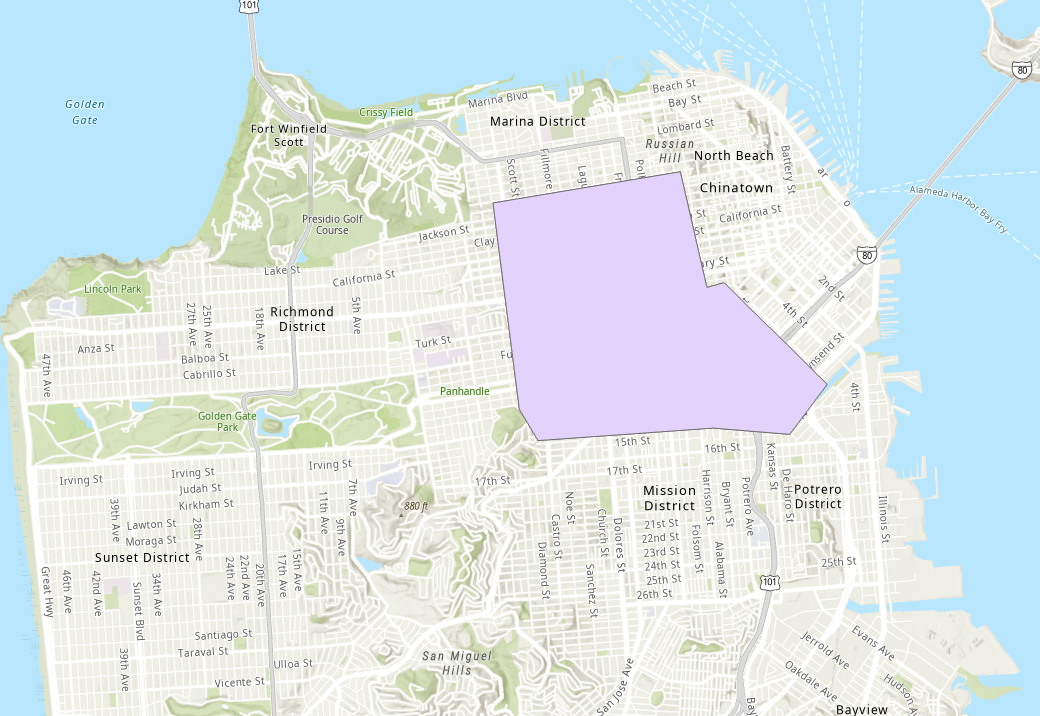
\includegraphics[width=14.44in]{image/san_fransisco_polygon_example} \caption{San Fransisco with example geofencing polygon.}\label{fig:sanfran-polygon}
\end{figure}

\begin{figure}
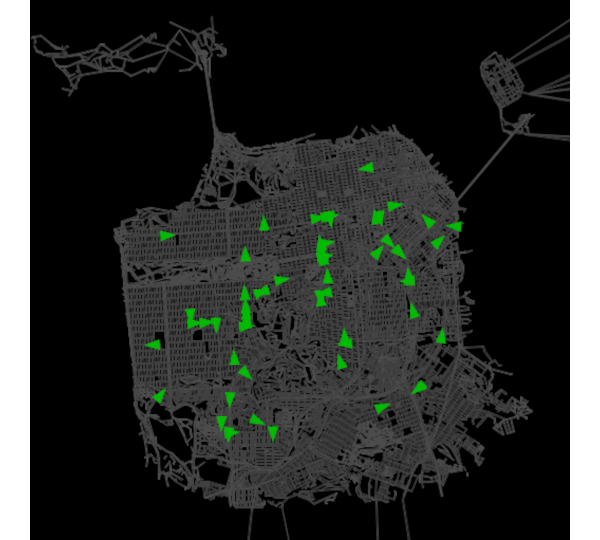
\includegraphics[width=0.5\linewidth]{image/all_vehicles_in_san_fransisco} 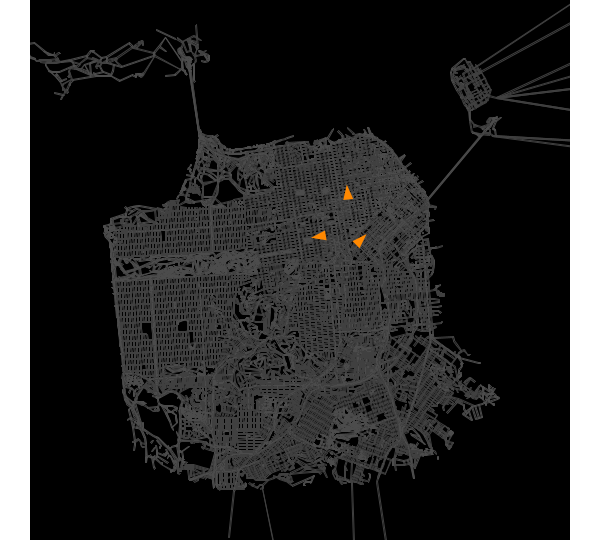
\includegraphics[width=0.5\linewidth]{image/odt_in_san_fransisco} \caption{Simulated vehicles in BEAM San Francisco scenario. Left: all vehicles (sample population). Right: ODT vehicles, restricted to user-specified operating area.}\label{fig:via-visualization}
\end{figure}

\hypertarget{scenario-description}{%
\subsection{Scenario Description}\label{scenario-description}}

The BEAM documentation (\protect\hyperlink{ref-beamdocs}{The BEAM Team, 2017}) lists the inputs required to run a BEAM scenario. Our implementation of BEAM largely follows these requirements, though there are a few differences. The following is a list of the requirements for our implementation:

\begin{itemize}
\tightlist
\item
  A configuration file
\item
  A population file
\item
  A households file and a corresponding attributes file
\item
  A plans file
\item
  A network
\item
  The definition of vehicle types
\item
  The personal vehicle fleet
\item
  The microtransit/ODT fleet
\item
  Transit data in the form of GTFS archives
\end{itemize}

These requirements are explained in greater detail in the following sections. For a full specification of the inputs, see the README at {[}\url{https://github.com/byu-transpolab/microtransit_areas2/README.md}{]}. Much of the work in creating these inputs was done by Macfarlane and Lant (\protect\hyperlink{ref-MacfarlaneLant}{2021}) previously, though we have made modifications to better fit our analysis.

\hypertarget{configuration-file}{%
\subsubsection{Configuration File}\label{configuration-file}}

The configuration file lists nearly all of the parameters used in the scenario, including aspects such as the number of iterations to run and paths to the other relevant files. This is one of the few input files that differs between the various scenarios we ran, as inputs such as the population and network remained constant. The configuration file is the main file that BEAM uses to set up and run the given scenario.

\hypertarget{population-and-household-files}{%
\subsubsection{Population and Household Files}\label{population-and-household-files}}

The population, households, and household attributes files are all part of a synthetic population created using PopulationSim. Macfarlane and Lant (\protect\hyperlink{ref-MacfarlaneLant}{2021}) generated this synthetic population in order to represent the WFRC/MAG region in 2019. We are using the same population in our analysis.

The population file consists of an identifier for each member of the population along with attributes such as age, income, and value of time. This file also contains the ID of the household to which each person belongs. The households and household attributes files contain information for each household in the population, including location, size, and auto ownership.

\hypertarget{plans-file}{%
\subsubsection{Plans File}\label{plans-file}}

We supplied the aforementioned synthetic population to the ActivitySim activity-based travel model platform, which created an initial travel demand in the form of a plans file. We set ActivitySim to model the demand for a single weekday. This plans file lists each person that made a trip during that day, as well as their corresponding plans, including information on the time, location, and nature of the attended activities, as well as the mode of transportation used for each leg of the trip.

\hypertarget{network-skims}{%
\paragraph{Network skims}\label{network-skims}}

In order to model destination choice and activity choice, ActivitySim requires network skims. We used the same skims as Macfarlane and Lant (\protect\hyperlink{ref-MacfarlaneLant}{2021}), which are modified from the skims in the existing WFRC trip-based model. These skims are not used directly in BEAM, however. A separate network file is required.

\hypertarget{network}{%
\subsubsection{Network}\label{network}}

Originally, we planned and attempted to use the network provided by Utah Geospatial Resource Center (\protect\hyperlink{ref-UGRCnetwork}{n.d.}) to create an ``all-streets'' network. However, we ran into several issues with this approach. One issue in particular was that of connectivity: in the provided network file, several roadways did not connect where they should and many highway overpasses were erroneously connected to the roads underneath, among other problems. Because of this, we instead used the network in the Wasatch Front Regional Council's travel demand model (\protect\hyperlink{ref-WFRCnetwork}{Wasatch Front Regional Council, n.d.}).

\hypertarget{vehicle-fleets-and-types}{%
\subsubsection{Vehicle Fleets and Types}\label{vehicle-fleets-and-types}}

Several files relate to the various vehicle fleets in the scenario. Central to these is a definition file containing the name and attributes of each vehicle type. We specified a personal vehicle fleet according to the auto ownership information given in the households file, and a microtransit/ODT fleet based on each of the scenarios we included. Section \ref{scenario-configuration} contains more information on the specific fleets we used.

Another aspect of this is assigning routes and schedules to transit vehicles. BEAM uses GTFS data for this. In our case, we used the GTFS archives provided by UTA, valid for March--April 2022. In our configuration we chose a specific date of March 30, 2022, which is a Wednesday.

\hypertarget{scenario-configuration}{%
\subsection{Scenarios}\label{scenario-configuration}}

We first needed to assess the performance of BEAM relative to real-world data. As UTA already has a microtransit ODT pilot program underway, we reached out to find the fleet size and shifts for the microtransit vehicles. Shaina Quinn, a researcher at UTA's Office of Innovative Mobility Solutions, informed us that typically 12 vehicles provide service at a time. We found the shifts on UTA's website for the service (\protect\hyperlink{ref-SLCSouth}{Utah Transit Authority, 2021}).

UTA reported several metrics, which are presented in Table \ref{tab:uta-metrics}. Much of the data in that report, however, is not necessarily representative, due to the COVID-19 pandemic and its onset in late March 2020. We also considered that the data for December was not necessarily valuable: since the service was new, people who would otherwise have used it may not have been accustomed to or even known about it. We therefore decided to use the average of the data from January through March as our benchmark.

\begin{table}

\caption{\label{tab:uta-metrics}Metrics Reported by UTA for the ODT Pilot Program in Salt Lake County}
\centering
\begin{tabular}[t]{lrrr}
\toprule
Month & Avg wkday ridership & Utilization & Avg wait time (minutes)\\
\midrule
DEC & 224 & 1.33 & 9.0\\
JAN & 334 & 2.00 & 11.0\\
FEB & 392 & 2.31 & 12.0\\
MAR & 316 & 1.88 & 11.0\\
APR & 275 & 1.52 & 10.0\\
\addlinespace
MAY & 105 & 0.67 & 8.0\\
JUN & 162 & 1.10 & 9.0\\
JUL & 155 & 1.10 & 9.0\\
AUG & 193 & 1.50 & 12.0\\
SEP & 214 & 1.60 & 12.0\\
\addlinespace
OCT & 200 & 1.70 & 13.0\\
NOV & 169 & 1.70 & 13.0\\
\textbf{Average} & \textbf{228} & \textbf{1.53} & \textbf{10.8}\\
\textbf{Average JAN--MAR} & \textbf{347} & \textbf{2.06} & \textbf{11.3}\\
\bottomrule
\end{tabular}
\end{table}

We created a scenario in BEAM to model this pilot program, and compared the results with the metrics reported by UTA. Our initial comparison showed that BEAM significantly over-predicted microtransit ridership and under-predicted wait times relative to the reported data. After calibrating several of BEAM's internal coefficients, the results more closely matched the observed data, and so we retained those calibrated values for all of the scenarios we ran. More information on the calibration process is given in Section \ref{scenario-calibration}.

In addition to modeling the existing pilot program, we created other scenarios to analyze. A map showing the areas we analyzed is given in Figure \ref{fig:zone-map}. For each of these areas we defined a microtransit fleet, including fleet size and operating hours, which can be seen in Table \ref{tab:zone-fleets}. The size of the fleet for each area was determined from population and employment, based on the actual fleet sizes for the South SL Co and Westside SLC areas. The operating hours were likewise copied from the existing service hours. We were less concerned with modeling each of these areas individually, but rather how the addition of another area would affect the whole. We therefore created several scenarios as combinations of these areas, which are given in Table \ref{tab:scenarios-info}.

Since the beginning of this project, UTA has started full-time microtransit service in the original pilot program area, as well as in the ``Westside SLC'' area. As such, we included both of these areas in our ``Existing'' scenario as well as most of the others. We also analyzed a ``Split'' scenario, in which the original south Salt Lake county area is divided into an east and west area.

\begin{figure}
\centering
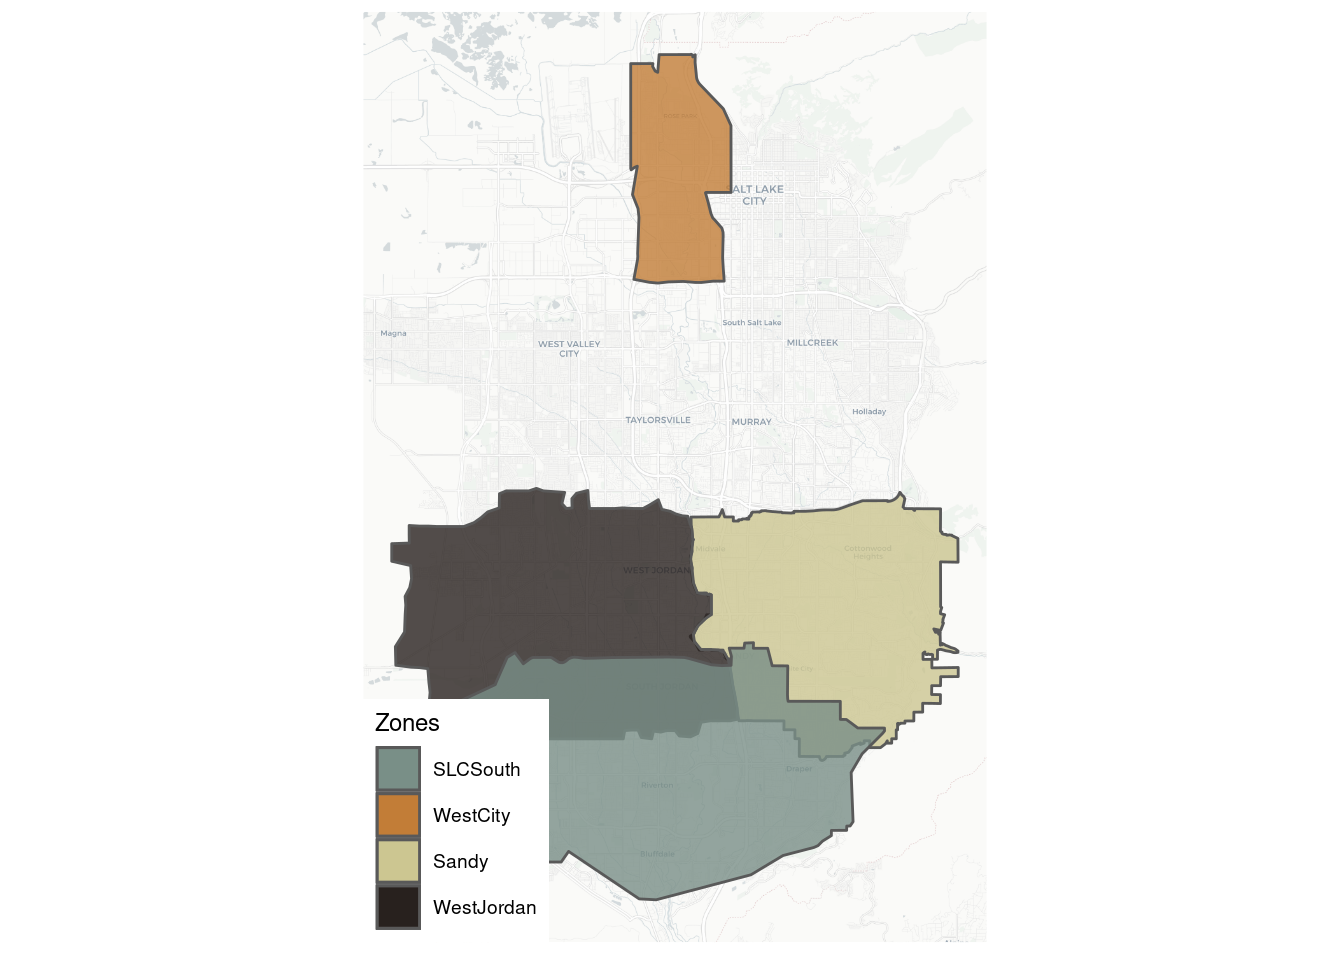
\includegraphics{microtransit_areas_files/figure-latex/zone-map-1.pdf}
\caption{\label{fig:zone-map}Map of areas studied.}
\end{figure}

\begin{table}

\caption{\label{tab:zone-fleets}Information on Fleets Used in Each Area}
\centering
\begin{tabular}[t]{lrrr}
\toprule
Area & Fleet Size & Shift Start (hour) & Shift End (hour)\\
\midrule
Westside SLC & 8 & 4 & 24.25\\
South SL Co & 17 & 4 & 24.25\\
South SL Co: East & 7 & 4 & 24.25\\
South SL Co: West & 14 & 4 & 24.25\\
Davis & 8 & 4 & 24.25\\
\addlinespace
Lehi & 7 & 4 & 24.25\\
Sandy & 16 & 4 & 24.25\\
\bottomrule
\end{tabular}
\end{table}

\begin{table}

\caption{\label{tab:scenarios-info}Areas Corresponding to Each Scenario}
\centering
\begin{tabular}[t]{ll}
\toprule
Name & Zones\\
\midrule
Existing & South SL Co, Westside SLC\\
Split & South SL Co: East, South SL Co: West, Westside SLC\\
EX + Davis & South SL Co, Westside SLC, Davis\\
EX + Lehi & South SL Co, Westside SLC, Lehi\\
EX + Sandy & South SL Co, Westside SLC, Sandy\\
\addlinespace
All & South SL Co, Westside SLC, Davis, Lehi, Sandy\\
\bottomrule
\end{tabular}
\end{table}

\hypertarget{common-configuration}{%
\subsubsection{Common configuration}\label{common-configuration}}

All of the scenarios we ran had a nearly identical configuration. The main exception to this was the ODT fleet used. There are many configurable options in BEAM (the full configuration is available at {[}\url{https://github.com/byu-transpolab/beam_scenarios}{]}), but there are two worth mentioning here: sample size and number of iterations.

Due to the computational power and time required to run BEAM, we were unable to run a full sample for any of our scenarios. We ultimately needed to decide on a balance between sample size and the number of iterations to run, as increasing one necessitated decreasing the other. We decided that 10 iterations was reasonable, as the smaller test scenarios seemed to mostly converge at that point. With 10 iterations, we were able to run a 20\% population sample for each of our scenarios. This sampling was done entirely in BEAM; BEAM offers support for this natively. BEAM also offers scaling factors for network capacity, which we set to match our population sample size.

However, we were not sure of the best, if any, way to scale the ODT fleets. We didn't simply scale the fleets to the same degree as the population, as that would create fleets containing a fractional number of vehicles. There was also a concern for availability: due to the small size of the fleets, there is no guarantee that there will be a vehicle available for any given ODT request. As such, it is not clear what the relationship between fleet size and ridership is, but it is not assumed to be a linear one.

\hypertarget{scenario-calibration}{%
\subsection{Calibration}\label{scenario-calibration}}

Ideally, the results of our model would match observed data when studying the same scenario. In our case, we used the mode shares as our metric. Our initial results significantly over-predicted ridehail usage, so we first looked to calibrate ActivitySim. BEAM takes the results of an ActivitySim model as an input, and so by adjusting ActivitySim to better reflect reality, calibrating BEAM became easier.

ActivitySim has several coefficients that can be changed to affect both tour and trip mode choice. We calibrated ActivitySim to about 1\% ridehail in the overall tour mode split. We then focused on calibrating the trip mode choice coefficients, but found that there was virtually no effect on overall mode split. Ultimately we were aiming for a 0.2\% ridehail mode share, which is less than what we were able to produce.

We then generated plans from ActivitySim again as our new input plans to BEAM. From there, we modified BEAM's coefficients in an attempt to again match our mode split target of 0.2\%, using a 15\% population sample. We were able to shift the mode split from its original values, but the results were similar to that of the ActivitySim calibration.

This sub-optimal calibration is a limitation of this study; however, we are generally more concerned with the relative performance between the scenarios we are studying rather than the absolute performance. This is discussed in more detail in Sections \ref{results} and \ref{recommendations}.

\hypertarget{results}{%
\section{Results}\label{results}}

\hypertarget{existing-scenario-evaluation}{%
\subsection{Existing scenario evaluation}\label{existing-scenario-evaluation}}

UTA, in partnership with VIA, ran a pilot program of microtransit service in south Salt Lake County from December 2019--November 2020. We also created a scenario in BEAM to model this pilot program. In order to assess the performance of our BEAM simulations when compared with real-world observed data, we compared the results of the two on several metrics (Table \ref{tab:existing-comparison}).

\begin{table}

\caption{\label{tab:existing-comparison}Comparison of Observed Data with 'Existing' BEAM Scenario}
\centering
\begin{tabular}[t]{lrrr}
\toprule
  & Ridership & Utilization & Avg. Wait Time (min)\\
\midrule
UTA Observed Data & 347 & 2.06 & 11.3\\
BEAM 'Pilot' Scenario & 314 & 1.29 & 10.1\\
\bottomrule
\end{tabular}
\end{table}

At first glance, these results seem to be quite good, as the simulated scenario reports similar ridership and wait time metrics to the real-world data. However, it is important to consider that our model scenario uses a 20\% population sample, and the observed data reflects the entire population. The model ODT fleet, on the other hand, was not scaled down to match the population sample size, and so represents the full fleet available in the real-world pilot program.

The fact that the predicted ridership and wait time is so similar to the actual, measured values is nevertheless encouraging. This suggests that the predicted ridership and wait times in the other modeled scenarios are a somewhat realistic forecast, albeit a rough approximation.

There is also a significant discrepancy in the utilization measurements. Because of the way utilization is calculated (passengers per hour per vehicle), the vehicle operating hours can greatly affect this metric. In our model scenario, all 12 of the ODT vehicles are operational nearly all day, and it is likely that in off-peak hours the actual pilot program had fewer vehicles available. If operating hours are taken to be only time that the ODT vehicles are in motion, then our modeled utilization becomes \textbf{TODO:} calculate this number.

\hypertarget{candidate-scenario-comparison}{%
\subsection{Candidate scenario comparison}\label{candidate-scenario-comparison}}

We then ran each of our scenarios as described in section \ref{scenario-configuration}, and compared several metrics. These metrics include total ridership, utilization, and wait time, as in the previous comparison, but also include \textbf{\emph{Other metrics}}. These comparisons are given in Table \ref{tab:scenario-compare}, and a plot of the wait times in Figure \ref{fig:wait-time-compare}.

\begin{table}

\caption{\label{tab:scenario-compare}Comparison Across BEAM Scenarios}
\centering
\begin{tabular}[t]{lrrrrrr}
\toprule
\multicolumn{5}{c}{ } & \multicolumn{2}{c}{Median Income (USD)} \\
\cmidrule(l{3pt}r{3pt}){6-7}
Scenario & Fleet Size & Ridership & Utilization & Avg. Wait Time (min) & ODT Users & Others\\
\midrule
Existing & 25 & 667 & 1.32 & 9.7 & 42266 & 53099\\
Split & 29 & 781 & 1.33 & 9.7 & 41831 & 53099\\
EX + Davis & 33 & 932 & 1.39 & 9.6 & 49555 & 53099\\
EX + Lehi & 32 & 833 & 1.29 & 9.7 & 41170 & 53099\\
EX + Sandy & 41 & 1079 & 1.30 & 9.6 & 42770 & 53099\\
\addlinespace
All & 56 & 1571 & 1.39 & 9.5 & 40919 & 53099\\
\bottomrule
\end{tabular}
\end{table}

It is clear that in the scenarios with more microtransit vehicles available, ridership greatly increases. Interestingly, utilization does not vary much at all, which implies that at least in these specific scenarios there is a roughly linear relationship between number of vehicles and number of riders. This relationship can also be seen in the ratios of passengers to fleet size, as all of the vehicle operating hours are identical. In fact, fitting a linear model to this data gives a predicted increase of about 29 passengers per ODT vehicle.

\begin{figure}
\centering
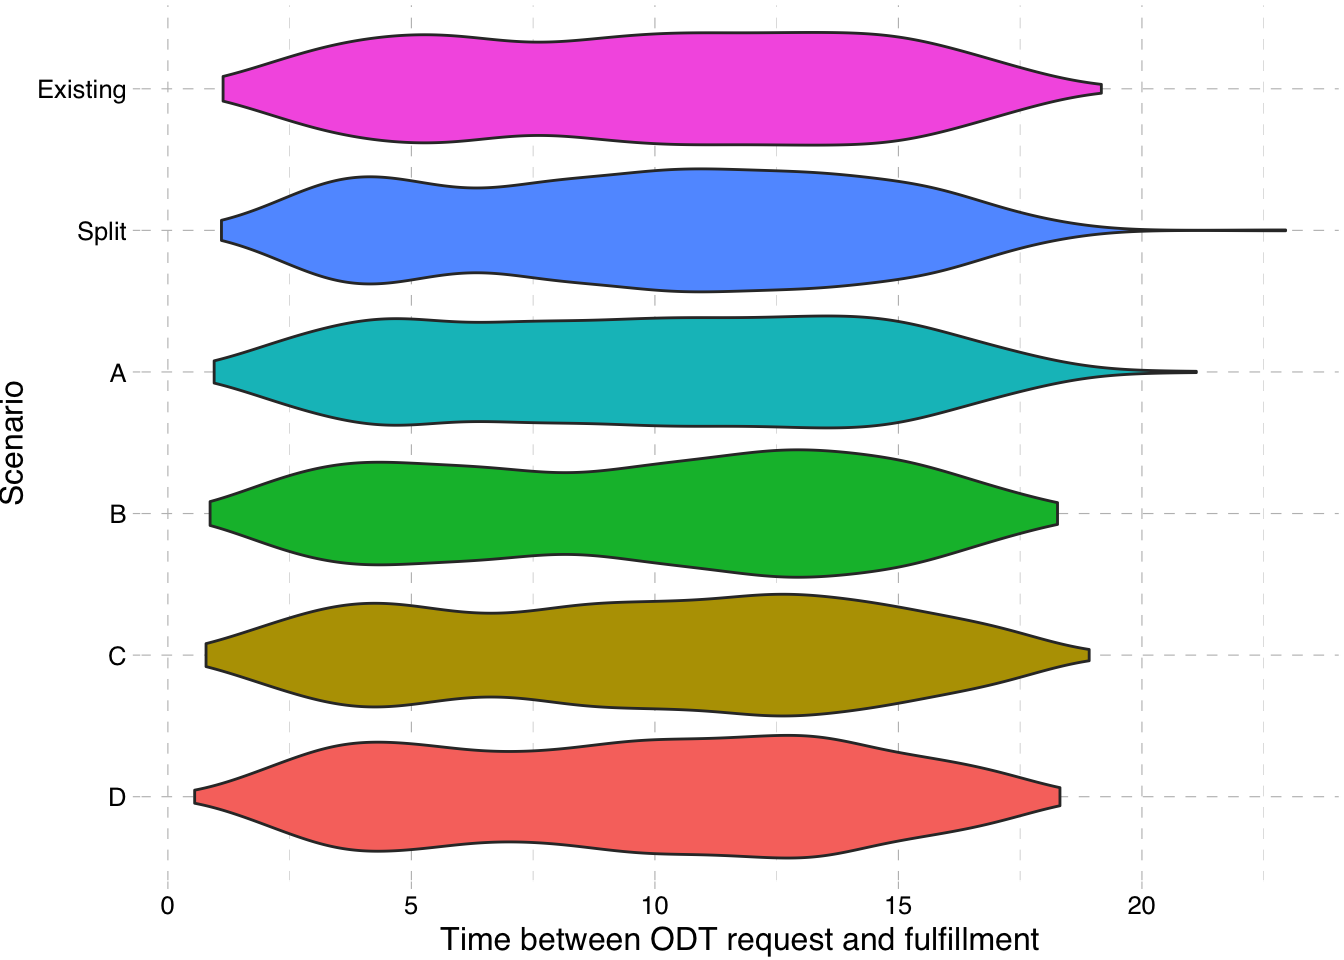
\includegraphics{microtransit_areas_files/figure-latex/wait-time-compare-1.pdf}
\caption{\label{fig:wait-time-compare}Comparison of ODT wait times in each scenario.}
\end{figure}

Wait times also hardly are affected in the various scenarios. Not only are the average wait times nearly identical between scenarios (as shown in Table \ref{tab:scenario-compare}), the distribution of wait times is essentially the same as well. It is important to note though that these wait times represent only \emph{fulfilled} ODT requests. In BEAM, when an agent makes an ODT request they may afterward re-plan and choose a different mode. Often this decision is largely based on the projected wait time for the ODT vehicle, so a request that returns a long wait time will often result in a change to mode choice. Table \ref{tab:odt-fulfillment} compares the proportion of fulfilled requests in each scenario.

\begin{table}

\caption{\label{tab:odt-fulfillment}Comparison of Fulfilled and Unfulfilled ODT Requests}
\centering
\begin{tabular}[t]{lrrrr}
\toprule
\multicolumn{1}{c}{} & \multicolumn{3}{c}{ODT Requests} & \multicolumn{1}{c}{} \\
\cmidrule(l{3pt}r{3pt}){2-4}
Scenario & Total & Fulfilled & Replanned & Proporiton Fulfilled\\
\midrule
Existing & 1066 & 642 & 424 & 0.602\\
Split & 1319 & 752 & 567 & 0.570\\
EX + Davis & 1633 & 899 & 734 & 0.551\\
EX + Lehi & 1419 & 801 & 618 & 0.564\\
EX + Sandy & 1850 & 1038 & 812 & 0.561\\
\addlinespace
All & 2605 & 1515 & 1090 & 0.582\\
\bottomrule
\end{tabular}
\end{table}

The proportion of ODT requests that were fulfilled also does not vary much between the scenarios. Notably, though, the values in the ``Existing'' and ``All'' scenarios are somewhat higher than the rest.

\hypertarget{summary-1}{%
\subsection{Summary}\label{summary-1}}

In these scenarios, we found that there is a roughly linear relationship between ridership and fleet size, and that utilization and wait times are essentially unaffected. Additionally, the differences between the ``Existing'' and ``Split'' scenarios were minimal. It appears that the demand for ODT service is a direct result of the supply; none of these scenarios are over-supplying ODT vehicles.

\hypertarget{recommendations}{%
\section{Recommendations}\label{recommendations}}

\hypertarget{overview-2}{%
\subsection{Overview}\label{overview-2}}

Will we ever run out of text?

\hypertarget{summary-2}{%
\subsection{Summary}\label{summary-2}}

Of course not

\hypertarget{references}{%
\section*{References}\label{references}}
\addcontentsline{toc}{section}{References}

\hypertarget{refs}{}
\begin{CSLReferences}{1}{0}
\leavevmode\vadjust pre{\hypertarget{ref-Agatz2011}{}}%
Agatz, N.A.H., Erera, A.L., Savelsbergh, M.W.P., Wang, X., 2011. Dynamic ride-sharing: A simulation study in metro atlanta. \emph{Transportation Research Part B: Methodological} 45 `, 1450--1464. \url{https://doi.org/10.1016/j.trb.2011.05.017}

\leavevmode\vadjust pre{\hypertarget{ref-Alonso-Gonzalez2018}{}}%
Alonso-González, M.J., Liu, T., Cats, O., Oort, N.V., Hoogendoorn, S., 2018. The potential of demand-responsive transport as a complement to public transport: An assessment framework and an empirical evaluation. \emph{Transportation Research Record: Journal of the Transportation Research Board} 2672, 879--889. \url{https://doi.org/10.1177/0361198118790842}

\leavevmode\vadjust pre{\hypertarget{ref-Azevedo2016}{}}%
Azevedo, C.L., Marczuk, K., Raveau, S., Soh, H., Adnan, M., Basak, K., Loganathan, H., Deshmunkh, N., Lee, D.-H., Frazzoli, E., Ben-Akiva, M., 2016. Microsimulation of demand and supply of autonomous mobility on demand. \emph{Transportation Research Record: Journal of the Transportation Research} 2564, 21--30. \url{https://doi.org/10.3141/2564-03}

\leavevmode\vadjust pre{\hypertarget{ref-Balac2015}{}}%
Balać, M.;, Ciari, F.;, Axhausen, K.W., 2015. Carsharing demand estimation zurich, switzerland, area case study. \emph{Transportation Research Record} 2536, 10--18. \url{https://doi.org/10.3929/ethz-b-000087032}

\leavevmode\vadjust pre{\hypertarget{ref-Bischoff2016}{}}%
Bischoff, J., Maciejewski, M., 2016. Simulation of city-wide replacement of private cars with autonomous taxis in berlin, in: Procedia Computer Science. Elsevier B.V., pp. 237--244. \url{https://doi.org/10.1016/j.procs.2016.04.121}

\leavevmode\vadjust pre{\hypertarget{ref-Buchanan2019}{}}%
Buchanan, M., 2019. The benefits of public transport. \emph{Nature Physics}. \url{https://doi.org/10.1038/s41567-019-0656-8}

\leavevmode\vadjust pre{\hypertarget{ref-Ciari2014}{}}%
Ciari, F., Bock, B., Balmer, M., 2014. Modeling station-based and free-floating carsharing demand. \emph{Transportation Research Record: Journal of the Transportation Research Board} 2416, 37--47. \url{https://doi.org/10.3141/2416-05}

\leavevmode\vadjust pre{\hypertarget{ref-Cyganski2018}{}}%
Cyganski, R., Heinrichs, M., Schmidt, A.V., Krajzewicz, D., 2018. Simulation of automated transport offers for the city of brunswick, in: Procedia Computer Science. Elsevier B.V., pp. 872--879. \url{https://doi.org/10.1016/j.procs.2018.04.083}

\leavevmode\vadjust pre{\hypertarget{ref-BEAMlbnl}{}}%
Energy Technologies Area, Berkeley Lab, n.d. {BEAM - the Modeling Framework for Behavior, Energy, Autonomy, and Mobility} {[}WWW Document{]}. URL \url{https://beam.lbl.gov}

\leavevmode\vadjust pre{\hypertarget{ref-Fagnant2014}{}}%
Fagnant, D.J., Kockelman, K.M., 2014. The travel and environmental implications of shared autonomous vehicles, using agent-based model scenarios. \emph{Transportation Research Part C: Emerging Technologies} 40, 1--13. \url{https://doi.org/10.1016/j.trc.2013.12.001}

\leavevmode\vadjust pre{\hypertarget{ref-Gershon2005}{}}%
Gershon, R.R.M., 2005. Public transportation: Advantages and challenges. \emph{Journal of Urban Health: Bulletin of the New York Academy of Medicine} 82. \url{https://doi.org/10.1093/jurban/jti003}

\leavevmode\vadjust pre{\hypertarget{ref-Heilig2015}{}}%
Heilig, M., Mallig, N., Schröder, O., Kagerbauer, M., Vortisch, P., 2015. Multiple-day agent-based modeling approach of station-based and free-floating carsharing.

\leavevmode\vadjust pre{\hypertarget{ref-Horni2016}{}}%
Horni, A., Nagel, K., Axhausen, K.W. (Eds.), 2016. The multi-agent transport simulation MATSim. Ubiquity Press. \url{https://doi.org/10.5334/baw}

\leavevmode\vadjust pre{\hypertarget{ref-MinetaTransportationInstitute2012}{}}%
Institute, M.T., 2012. \href{http://transweb.sjsu.edu}{The benefits of transit in the united states: A review and analysis of benefit-cost studies}.

\leavevmode\vadjust pre{\hypertarget{ref-Kang2019}{}}%
Kang, S., Hamidi, S., 2019. On-demand microtransit for better transit station and job accessibility.

\leavevmode\vadjust pre{\hypertarget{ref-Kari2016}{}}%
Kari, R., 2016. \href{https://www.hsl.fi}{Kutsuplus-final report helsinki regional transport authority (HSL)}.

\leavevmode\vadjust pre{\hypertarget{ref-MacfarlaneLant}{}}%
Macfarlane, G.S., Lant, N.J., 2021. \href{https://rosap.ntl.bts.gov/view/dot/56982}{Estimation and simulation of daily activity patterns for individuals using wheelchairs} (No. UT-21.10).

\leavevmode\vadjust pre{\hypertarget{ref-UTAreport}{}}%
Robertson, J., Callison, E., Taylor, R., 2020. \href{https://www.rideuta.com/-/media/Files/About-UTA/Reports/2021/UTA_Microtransit_Consulting_Report_Final.ashx?la=en}{{Utah Transit Authority Microtransit Planning Project}}.

\leavevmode\vadjust pre{\hypertarget{ref-Ronald2015}{}}%
Ronald, N., Thompson, R., Winter, S., 2015. Simulating demand-responsive transportation: A review of agent-based approaches. \emph{Transport Reviews} 35, 404--421. \url{https://doi.org/10.1080/01441647.2015.1017749}

\leavevmode\vadjust pre{\hypertarget{ref-Schofer2003}{}}%
Schofer, J.L., Nelson, B.L., Eash, R., Daskin, M., Yang, Y., Wan, H., Yan, J., Medgyesy, L., 2003. \href{http://www.national-academies.org/trb/bookstore}{Resource requirements for demand-responsive transportation services}. Michael S. Townes, President; CEO.

\leavevmode\vadjust pre{\hypertarget{ref-Shaheen2015}{}}%
Shaheen, S., Chan, N., Bansal, A., Cohen, A., Shaheen, S., Chan, N., Bansal, A., Cohen, A., Berkeley, U., Alm, E., Grimes, A., Huckabay, L., Iacobucci, L., Morneau, J., Longoria, N., Schermer, F., Srivastava, R., Williams, S., 2015. Definitions, industry developments, and early understanding ACKNOWLEDGEMENTS.

\leavevmode\vadjust pre{\hypertarget{ref-SimuntoVIA}{}}%
Simunto GmbH, n.d. VIA features {[}WWW Document{]}. URL \url{https://www.simunto.com/via/} (accessed 10.4.2022).

\leavevmode\vadjust pre{\hypertarget{ref-beamdocs}{}}%
The BEAM Team, 2017. {BEAM Documentation} {[}WWW Document{]}. URL \url{https://beam.readthedocs.io/en/latest/about.html} (accessed 11.11.2021).

\leavevmode\vadjust pre{\hypertarget{ref-UTAevalQ1}{}}%
UTA Innovative Mobility Solutions, 2021a. \href{https://www.rideuta.com/-/media/Files/Services/Via/Final_UTA_microtransit_pilot_Q1_report.ashx?la=en}{{Utah Transit Authority Quarterly Microtransit Pilot Project Evaluation (Q1)}}.

\leavevmode\vadjust pre{\hypertarget{ref-UTAevalQ2}{}}%
UTA Innovative Mobility Solutions, 2021c. \href{https://www.rideuta.com/-/media/Files/Services/Via/Final_UTA_Microtransit_Pilot_Q2_Report.ashx?la=en}{{Utah Transit Authority Quarterly Microtransit Pilot Project Evaluation (Q2)}}.

\leavevmode\vadjust pre{\hypertarget{ref-UTAevalQ3}{}}%
UTA Innovative Mobility Solutions, 2021b. \href{https://www.rideuta.com/-/media/Files/Services/Via/Final_UTA_Microtransit_Pilot_Q3_Report.ashx?la=en}{{Utah Transit Authority Quarterly Microtransit Pilot Project Evaluation (Q3)}}.

\leavevmode\vadjust pre{\hypertarget{ref-UTAevalDEC}{}}%
UTA Innovative Mobility Solutions, 2019. \href{https://www.rideuta.com/-/media/Files/About-UTA/Reports/Via/Microtransit_Evaluation_Dec_2019.ashx}{{Utah Transit Authority Quarterly Microtransit Pilot Project Evaluation (Q1)}}.

\leavevmode\vadjust pre{\hypertarget{ref-UGRCnetwork}{}}%
Utah Geospatial Resource Center, n.d. Street network analysis {[}WWW Document{]}. URL \url{https://gis.utah.gov/data/transportation/street-network-analysis/\#StreetNetwork} (accessed 11.11.2021).

\leavevmode\vadjust pre{\hypertarget{ref-SLCSouth}{}}%
Utah Transit Authority, 2021. \href{https://www.rideuta.com/Services/UTA-On-Demand/Southern-Salt-Lake-County}{{Southern Salt Lake County}}.

\leavevmode\vadjust pre{\hypertarget{ref-Viergutz2019}{}}%
Viergutz, K., Schmidt, C., 2019. Demand responsive - vs. Conventional public transportation: A MATSim study about the rural town of colditz, germany, in: Procedia Computer Science. Elsevier B.V., pp. 69--76. \url{https://doi.org/10.1016/j.procs.2019.04.013}

\leavevmode\vadjust pre{\hypertarget{ref-Vosooghi2017}{}}%
Vosooghi, R., Puchinger, J., Jankovic, M., Sirin, G., 2017. \href{https://hal.archives-ouvertes.fr/hal-01622293}{A critical analysis of travel demand estimation for new one-way carsharing systems}. IEEE.

\leavevmode\vadjust pre{\hypertarget{ref-WFRCnetwork}{}}%
Wasatch Front Regional Council, n.d. Wasatch front travel demand model {[}WWW Document{]}. URL \url{https://wfrc.org/programs/models-forecasting} (accessed 11.11.2021).

\end{CSLReferences}

\end{document}
